\documentclass[10pt,a4paper,onecolumn,notitlepage]{article}
\usepackage{IEEEtrantools}
\usepackage[parfill]{parskip}
\usepackage{amsmath}
\usepackage{graphicx}
\usepackage{algorithmicx,algpseudocode}
\usepackage[per-mode=symbol]{siunitx}
\usepackage[usenames,dvipsnames,svgnames,table]{xcolor}
\usepackage{listings}
\lstset{basicstyle=\ttfamily\footnotesize,
	breaklines=true,
	keywordstyle=\color{blue}\bf,
    commentstyle=\color{OliveGreen},
    stringstyle=\color{red},
    numbers=left,
    numberstyle=\tiny,
    numbersep=5pt,}
\lstset{language=MATLAB}
\lstset{language=C++}
%\usepackage[pdftex]{hyperref}
%\usepackage[all]{hypcap}
\usepackage[nameinlink, capitalize]{cleveref}

\title{SPINE Manual}
\author{J.P.G. van Dijk}

\begin{filecontents}{spine.bib}
	
	@IEEEtranBSTCTL{IEEEexample:BSTcontrol,
		CTLdash_repeated_names   = "no",
	}
	
	@InProceedings{van2018co,
  		author       = {Jeroen van Dijk and Andrei Vladimirescu and Masoud Babaie and Edoardo Charbon and Fabio Sebastiano},
  		title        = {A co-design methodology for scalable quantum processors and their classical electronic interface},
  		booktitle    = {2018 Design, Automation {\&} Test in Europe Conference {\&} Exhibition ({DATE})},
  		year         = {2018},
  		organization = {IEEE},
  		publisher    = {{IEEE}},
  		month        = {mar},
  		pages        = {573--576},
  		doi          = {10.23919/date.2018.8342072},
  		url          = {\url{https://ieeexplore.ieee.org/document/8342072}},
	}

	@InProceedings{van2019spine,
	  author       = {Jeroen van Dijk and Andrei Vladimirescu and Masoud Babaie and Edoardo Charbon and Fabio Sebastiano},
	  title        = {{SPINE} ({SPIN} Emulator) - A Quantum-Electronics Interface Simulator},
	  booktitle    = {2019 {IEEE} 8th International Workshop on Advances in Sensors and Interfaces ({IWASI})},
	  year         = {2019},
	  organization = {IEEE},
	  publisher    = {{IEEE}},
	  month        = {jun},
	  pages        = {23--28},
	  doi          = {10.1109/iwasi.2019.8791334},
	  url          = {\url{https://ieeexplore.ieee.org/document/8791334}},
	}

	@Article{van2019impact,
	  author    = {J.P.G. van Dijk and E. Kawakami and R.N. Schouten and M. Veldhorst and L.M.K. Vandersypen and M. Babaie and E. Charbon and F. Sebastiano},
	  title     = {Impact of Classical Control Electronics on Qubit Fidelity},
	  journal   = {Physical Review Applied},
	  year      = {2019},
	  volume    = {12},
	  number    = {4},
	  month     = {oct},
	  pages     = {044054},
	  doi       = {10.1103/physrevapplied.12.044054},
	  publisher = {American Physical Society ({APS})},
	  url       = {\url{https://journals.aps.org/prapplied/abstract/10.1103/PhysRevApplied.12.044054}}
	}

	@Article{veldhorst2015two,
	  author    = {M. Veldhorst and C. H. Yang and J. C. C. Hwang and W. Huang and J. P. Dehollain and J. T. Muhonen and S. Simmons and A. Laucht and F. E. Hudson and K. M. Itoh and A. Morello and A. S. Dzurak},
	  title     = {A two-qubit logic gate in silicon},
	  journal   = {Nature},
	  year      = {2015},
	  volume    = {526},
	  number    = {7573},
	  month     = {oct},
	  pages     = {410--414},
	  note      = {Letter},
	  issn      = {0028-0836},
	  doi       = {10.1038/nature15263},
	  day       = {15},
	  publisher = {Springer Science and Business Media {LLC}},
	}

	@article{gonzalez2015probing,
		title={Probing the limits of gate-based charge sensing},
		author={Gonzalez-Zalba, MF and Barraud, S and Ferguson, AJ and Betz, AC},
		journal={Nature communications},
		volume={6},
		pages={6084},
		year={2015},
		publisher={Nature Publishing Group}
	}

\end{filecontents}

\begin{document}
\bstctlcite{IEEEexample:BSTcontrol}

\maketitle
\tableofcontents
\clearpage

\section{Introduction}
SPINE -- SPIN Emulator -- is a tool for the co-simulation of classical electrical signals with spin-based quantum processors, and was originally introduced in \cite{van2018co,van2019spine}. The tool was extensively used in deriving the impact of classical control electronics on the fidelity of a single-electron spin qubit \cite{van2019impact}. However, the toolset can be directly extended to other qubit technologies.

\subsection{Simulation Platforms}
The simulator is implemented in different platforms, with different features/limitations as discussed in the following.

\subsubsection{MATLAB}
As SPINE was originally written in MATLAB, this implementation contains all features present in the other platforms. Leveraging the power of MATLAB, it has better plotting functions (e.g., 3D plot) and additional solvers (\lstinline{solver_expm}, \lstinline{solver_taylor_sparse_approx}).

This implementation was tested on Windows 10 Pro 64-bit (1903) running MATLAB R2018a 64-bit.

\subsubsection{C++}
The C++ implementation of the simulator can in principle be used on any host OS, without the need for MATLAB to be installed on the system. Additionally, by defining \lstinline{MKL}, the Intel\textsuperscript{\textcopyright} Math Kernel Library (with or without multi-threading [requires MPI]) is used to optimize most calculations. Moreover, there is explicit control over the used precision, with single precision floating point arithmetic the default, unless \lstinline{DOUBLE_PRECISION} is defined (advised). Finally, when running on Microsoft Windows, plotting functions are available, which can be enabled by defining \lstinline{PLOT}. All matrices are stored in row-major order.

This implementation was tested on Windows 10 Pro 64-bit (1903) with MKL version 2019.5.281, compiled using Visual Studio 2017 (v141) and Windows SDK Version 10.0.17763.0.

\subsubsection{Verilog-A}
The Verilog-A implementation is meant for the simulation of the quantum processor in an electrical circuit simulator supporting Verilog-A models. Because of the limitations of the Verilog-A language, only the following modules are available:
\begin{itemize}
	\item \lstinline{spine_qubit1}: a port of the simulator for one single-electron spin qubit in the lab frame (\lstinline{system_1_spin}) solved using the available analytical solution (\lstinline{solver_analytical_xz}).
	\item \lstinline{spine_qubit2}: a port of the simulator for two single-electron spin qubits, each with singlet state (\lstinline{system_2_spin_2_singlet}), solved using a Taylor series expansion (\lstinline{solver_taylor}).
\end{itemize}

This implementation was tested on a CentOS 5.11 server (linux kernel 2.6.18-410.el5) running Cadence\textsuperscript{\textregistered} IC6.1.5.500.6 (32-bit) with Spectre version 7.2.0.307.isr10.

More details of the Verilog-A implementation can be found in \cref{sec:veriloga}.

\section{SPINE}

\subsection{Hamiltonian Simulation}
The evolution of the quantum processor's state, captured as a vector $|\psi\rangle$, can be described by the multiplication with a unitary matrix $U$: $|\psi(t)\rangle = U \cdot |\psi(0)\rangle$. In general, finding this operation $U$ involves solving the time-dependent Schr\"{o}dinger equation:
\begin{equation}
\mathrm{i} \hbar \cdot \frac{\partial|\psi(t)\rangle}{\partial t} = H(t) \cdot |\psi(t)\rangle,
\end{equation}
where $H(t)$ is the Hamiltonian describing the system. In general, an approximate solution can be more easily found by simulation. Such a Hamiltonian simulation relies on the fact that the solution to a time-independent Hamiltonian $H_n$ is trivially:
\begin{equation}
U_n = \mathrm{e}^{-\mathrm{i}/\hbar \cdot H_n \cdot t}.
\end{equation}
Then, by approximating the time-dependent Hamiltonian as many time-independent Hamiltonians $H_n$ that are valid only for a short duration $t$, which are all applied subsequently, the overall operation can be found:
\begin{equation}
U_{\mathrm{overall}} = \prod_{n=N}^{1} U_n = U_N \cdot \cdots \cdot U_2 \cdot U_1.
\end{equation}
This process is called trotterization. Note that the order of the matrix multiplication matters. Moreover, for simplicity $\hbar = 1$ throughout SPINE.

\subsection{SPINE Simulator Core}
The pseudo-code of the core of the SPINE simulator is shown below:
\begin{algorithmic}
\Function{simulate}{$inHamiltonian$, $outOperation$, $solver$}
	\State $U\gets I$
	\While{$inHamiltonian$($H$, $dt$)}
		\State $dU \gets$ \Call{$solver$}{$H \cdot dt$}
		\State $U \gets dU \cdot U$
		\State \Call{$outOperation$}{$U$}
	\EndWhile
\EndFunction
\end{algorithmic}
This function calculates the overall operation $U$ at any time, given the user-provided Hamiltonian $H$ and time step $dt$ at that time (through the callback function $\mathit{inHamiltonian}$) and passes the resulting $U$, at that time, back to the user (through the callback function $\mathit{outOperation}$). The user needs to provide a $\mathit{solver}(\mathrm{arg})$ that calculates $\mathrm{e}^{-\mathrm{i} \cdot \mathrm{arg}}$.

If instead of a simulation of the full quantum operation, only a simulation of the quantum state is desired, the faster simulation as shown below is executed:
\begin{algorithmic}
	\Function{simulate}{$inHamiltonian$, $outOperation$, $solver$, $state$}
	\While{$inHamiltonian$($H$, $dt$)}
	\State $dU \gets$ \Call{$solver$}{$H \cdot dt$}
	\State $state \gets dU \cdot state$
	\State \Call{$outOperation$}{$state$}
	\EndWhile
	\EndFunction
\end{algorithmic}
This function calculates the quantum state $state$ at any time, given the user-provided Hamiltonian $H$ and time step $dt$ at that time (through the callback function $\mathit{inHamiltonian}$) and passes the resulting $state$, at that time, back to the user (through the callback function $\mathit{outOperation}$). The user needs to provide a $\mathit{solver}(\mathrm{arg})$ that calculates $\mathrm{e}^{-\mathrm{i} \cdot \mathrm{arg}}$.

The advantages of such a generic setup using callbacks are as follows:
\begin{itemize}
	\item Allows for dynamic time step size.
	\item There is no requirement for a predetermined number of points or simulation time.
	\item There is no requirement for a predetermined signal; it can be generated based on previous simulation points if desired.
	\item There is freedom in what to do with the simulated operation/state at any time instance, e.g.~plot or save every N\textsuperscript{th} point.
\end{itemize}

\subsection{Functions}

\subsubsection{\lstinline{simulate}}
The function prototype of $\mathit{simulate}$ in MATLAB and C++, respectively, is:
\begin{lstlisting}[language=MATLAB]
function simulate(dim, inHamiltonian, outOperation, solver, varargin)
\end{lstlisting}
\begin{lstlisting}[language=C++]
void simulate(unsigned int dim,
	bool(*inHamiltonian)(complex * H, realnum * dt),
	void(*outOperation)(complex * U),
	void(*solver)(unsigned int dim, complex * H, complex * dU));
void simulate(unsigned int dim,
	bool(*inHamiltonian)(complex * H, realnum * dt),
	void(*outOperation)(complex * U),
	void(*solver)(unsigned int dim, complex * H, complex * dU),
	complex * state);
\end{lstlisting}
The dimension of the Hamiltonian should be passed in \lstinline{dim}. Additionally, handles to the functions \lstinline{inHamiltonian}, \lstinline{outOperation} and \lstinline{solver} should be passed.
For the C++ implementation, additional optimized functions are available when using real-valued Hamiltonians (\lstinline{arg} is real). In both the MATLAB and C++ implementation, an additional optional argument \lstinline{state} can be passed in which case only the quantum state evolution, instead of the full quantum operation, is simulated, assuming initial state \lstinline{state}. 

\subsubsection{\lstinline{inHamiltonian}}
The function prototype of $\mathit{inHamiltonian}$ in MATLAB and C++, respectively, is:
\begin{lstlisting}[language=MATLAB]
function [run, H, dt] = inHamiltonian()
\end{lstlisting}
\begin{lstlisting}[language=C++]
bool inHamiltonian(complex * H, realnum * dt);
\end{lstlisting}
For the MATLAB implementation, \lstinline{run}, specifies whether the simulation should continue or not, whereas this is returned as boolean variable in the C++ implementation.
For the C++ implementation, the memory regions passed as arguments (\lstinline{H} and \lstinline{dt}) are filled by the function \lstinline{inHamiltonian}. For the C++ implementation, an additional optimized function is available when using real-valued Hamiltonians.

Several Hamiltonians for different spin systems are provided in the MATLAB package \lstinline{spine.systems} and the C++ namespace \lstinline{spine::systems}. For more information, see \cref{sec:systems}.

\subsubsection{\lstinline{outOperation}}
The function prototype of $\mathit{outOperation}$ in MATLAB and C++, respectively, is:
\begin{lstlisting}[language=MATLAB]
function outOperation(U)
\end{lstlisting}
\begin{lstlisting}[language=C++]
void outOperation(complex * U);
\end{lstlisting}

Several helper functions for plotting the operation/state and calculating the fidelity of the operation are provided in MATLAB as \lstinline{spine.plot*()} and \lstinline{spine.fidelity()}), respectively, and in C++ as \lstinline{spine::Plot()} and \lstinline{spine::fidelity()}, respectively. For more information, see \cref{sec:helper}.

\subsubsection{\lstinline{solver}}
The function prototype of $\mathit{solver}$ in MATLAB and C++, respectively, is:
\begin{lstlisting}[language=MATLAB]
function dU = solver(dim, arg)
\end{lstlisting}
\begin{lstlisting}[language=C++]
void solver(unsigned int dim, complex * arg, complex * dU);
\end{lstlisting}
The dimension of the argument \lstinline{arg} should be passed in \lstinline{dim}.
For the C++ implementation, the memory region passed as argument (\lstinline{dU}) is filled by the function \lstinline{solver}. For the C++ implementation, additional optimized functions are available when using real-valued Hamiltonians (\lstinline{arg} is real).

Several solvers are provided in the MATLAB package \lstinline{spine.solvers} and the C++ namespace \lstinline{spine::solvers}. For more information, see \cref{sec:solvers}.

\section{Implemented Spin Systems}
\label{sec:systems}
For the simulation of single-qubit gates on an isolated quantum dot, a good approximation is obtained when only considering the spin-up and spin-down states of the electron, i.e.: $|\psi\rangle = \alpha_0 \cdot |\mathord{\uparrow}\rangle + \alpha_1 \cdot |\mathord{\downarrow}\rangle$, where $|\mathord{\uparrow}\rangle$ and $|\mathord{\downarrow}\rangle$ can be considered the qubit states $|\mathord{0}\rangle$ and $|\mathord{1}\rangle$ respectively. The state vector only contains 2 complex numbers, and the matrices involved in the simulation are $2 \times 2$.

The Hamiltonian of the spin qubit with the energy levels split by the Zeeman energy $\hbar \omega_0$ under excitation by a signal $x(t)$ in a perpendicular magnetic field is given by (setting $\hbar = 1$):
\begin{equation}
H(t) = -\omega_0 \frac{\sigma_z}{2} + x(t) \frac{\sigma_x}{2}
\end{equation}
where $\sigma_x$ and $\sigma_z$ are the X and Z Pauli matrices. In general, the signal $x(t)$ is a sinusoidal signal with frequency $\omega_0$ and varying amplitude.

For the simulation of two qubits, it would seem sufficient to simply take the qubit state as $|\psi\rangle = \alpha_{00} \cdot |\mathord{\uparrow\uparrow}\rangle + \alpha_{01} \cdot |\mathord{\uparrow\downarrow}\rangle + \alpha_{10} \cdot |\mathord{\downarrow\uparrow}\rangle + \alpha_{11} \cdot |\mathord{\downarrow\downarrow}\rangle$ with a Hamiltonian $H = H_A \oplus H_B$ where $H_i$ describes the physics of a single quantum dot. This is indeed sufficient for the simulation of single-qubit operations on multiple isolated qubits. However, for the simulation of two-qubit gates at least one more energy level should be included in the simulation that is responsible for the qubit interactions in the physical system:
$|\psi\rangle = \alpha_{00} \cdot |\mathord{\uparrow\uparrow}\rangle + \alpha_{01} \cdot |\mathord{\uparrow\downarrow}\rangle + \alpha_{10} \cdot |\mathord{\downarrow\uparrow}\rangle + \alpha_{11} \cdot |\mathord{\downarrow\downarrow}\rangle + \alpha_{S0} \cdot |\mathord{S0}\rangle$
where $|\mathord{S0}\rangle$ describes the lowest energy state (a Singlet state) where both electrons have moved into one of the quantum dots. The corresponding system Hamiltonian, now also of size $5 \times 5$, is given by \cite{veldhorst2015two}:
\begin{equation}
H = \begin{bmatrix}
-\frac{\omega_{0,A} + \omega_{0,B}}{2} & 0 & 0 & 0 & 0\\
0 & -\frac{\omega_{0,A} - \omega_{0,B}}{2} & 0 & 0 & t_0\\
0 & 0 & \frac{\omega_{0,A} - \omega_{0,B}}{2}  & 0 & -t_0\\
0 & 0 & 0 & \frac{\omega_{0,A} + \omega_{0,B}}{2}  & 0\\
0 & t_0 & -t_0 & 0 & U-\epsilon
\end{bmatrix}
\end{equation}
where for simplicity the driving term $x(t)$ has been left out. The tunnel coupling $t_0$ and detuning $\epsilon$ are generally time-varying signals. This Hamiltonian allows for the simulation of the controlled-Z gate at a detuning ($\epsilon \approx U$).

However, for the simulation of e.g. a controlled-Z gate at no detuning, or a SWAP gate, the state vector has to be expanded with the $|\mathord{0S}\rangle$ state, describing that both electrons can also go into the other quantum dot. For more accurate simulations, as also required for the simulation of a qubit measurement by pauli-spin blockade, even higher energy levels have to be included.

Due to the fact that it is not sufficient to only simulate two energy levels for a single quantum bit, the simulation complexity grows very rapidly for larger qubit
systems. Considering an isolated system (the number of electrons does not change), where only the lowest states with 2 electrons in a single dot are considered (the Singlet states), the length of the state vector grows as:

\begin{tabular}{ll}
	Qubits & Dimension \\
	\hline
	2 & 6 \\
	3 & 20 \\
	4 & 70 \\
	5 & 252 \\
	6 & 924
\end{tabular}

In MATLAB the following systems are currently available for simulation (in the package \lstinline{spine.systems}):
\begin{itemize}
	\item \lstinline{spine.systems.system_spin}
		\begin{itemize}
			\item \lstinline{spine.systems.system_1_spin}
			\item \lstinline{spine.systems.system_1_spin_rwa}
			\item \lstinline{spine.systems.system_2_spin_1_singlet}
			\item \lstinline{spine.systems.system_2_spin_2_singlet}
			\item \lstinline{spine.systems.system_2_spin_1_singlet_triplet}
			\item \lstinline{spine.systems.system_2_spin_2_singlet_triplet}
			\item \lstinline{spine.systems.system_n_spin_n_singlet}
		\end{itemize}
	\item \lstinline{spine.systems.system_1_singlet_triplet}
	\item \lstinline{spine.systems.system_dispersive_readout}

\end{itemize}
In C++ the following systems are currently available for simulation (in the namespace \lstinline{spine::systems}):
\begin{itemize}
	\item \lstinline{spine::systems::system_spin}
		\begin{itemize}
			\item \lstinline{spine::systems::system_1_spin}
			\item \lstinline{spine::systems::system_1_spin_rwa}
			\item \lstinline{spine::systems::system_2_spin_1_singlet}
			\item \lstinline{spine::systems::system_2_spin_2_singlet}
			\item \lstinline{spine::systems::system_2_spin_1_singlet_triplet}
			\item \lstinline{spine::systems::system_2_spin_2_singlet_triplet}
			\item \lstinline{spine::systems::system_n_spin_n_singlet}
		\end{itemize}
	\item \lstinline{spine::systems::system_1_singlet_triplet}
	\item \lstinline{spine::systems::system_dispersive_readout}
\end{itemize}

\subsection{\lstinline{system_spin}}
\label{sec:system_spin}
Each of the \lstinline{system_*_spin} classes is derived from the \lstinline{system_spin} base class that contains most of the functionality for simulating any number of \emph{single-electron spin qubits} with any number of energy levels per dot considered (the 0 and 1 computational states, with optional singlet and triplet energy levels).

This base class contains the storage and general getters/setters for the Hamiltonian properties (Larmor frequency, Rabi frequency, charging energy, singlet-triplet energy splitting) and control variables (microwave signal, detuning signal, tunnel control signal) for every dot.

Additionally, it contains helper functions \lstinline{initialize} and \lstinline{measure} (\lstinline{measureST}) to initialize a state vector to the ground state of the system and to measure the state of every qubit in the X,Y,Z basis (or the singlet and triplet occupancy probability of the dot), respectively. Optionally, a time $t$ can be passed to the function \lstinline{measure} to measure the state in the rotating frame at time $t$ instead of the lab frame. These functions, however, rely on an implementation of the following functions in the derived class:
\begin{itemize}
	\item \lstinline{getIndex}: given the desired state of every quantum dot, passed as argument, returns the corresponding index in the state vector/Hamiltonian.
	\item \lstinline{getIndexMeasurement}: given a dot and the state of interest, passed as argument, returns all indices in the state vector/Hamiltonian where that dot is in the desired state.
	\item \lstinline{getDimension}: returns the dimension of the state vector/Hamiltonian.
\end{itemize}
On top of the \lstinline{measure} functions, additional \lstinline{plot} functions are provided to plot the X,Y,Z measurement probability for every dot in a Bloch sphere (MATLAB) or a simple 2D plot (C++, Windows only), see \cref{sec:helper}.

\subsubsection{\lstinline{system_1_spin}}
This class contains the $2\times2$ real-valued Hamiltonian of 1 single-electron spin-qubit in a single quantum dot, considering only the energy levels of the 0 and 1 states.

\subsubsection{\lstinline{system_1_spin_rwa}}
This class contains the $2\times2$ complex Hamiltonian of 1 single-electron spin-qubit in a single quantum dot, in the rotating frame with rotating wave approximation, considering only the energy levels of the 0 and 1 states.

\subsubsection{\lstinline{system_2_spin_1_singlet}}
This class contains the $5\times5$ real-valued Hamiltonian of 2 single-electron spin-qubits in a double quantum dot, considering only the energy levels of the 0 and 1 states. Additionally, the singlet state energy level of one of the dots is included to allow for basic 2-qubit operations. For simplicity, a single microwave drive line and a common Rabi frequency is assumed for the two dots.

\subsubsection{\lstinline{system_2_spin_2_singlet}}
This class contains the $6\times6$ real-valued Hamiltonian of 2 single-electron spin-qubits in a double quantum dot, considering the energy levels of the 0 and 1 states, and the singlet state for both quantum dots. For simplicity, a single microwave drive line and a common Rabi frequency and charging energy are assumed for the two dots. Moreover, only the relative detuning of the two dots is considered.

\subsubsection{\lstinline{system_2_spin_1_singlet_triplet}}
This class contains the $8\times8$ real-valued Hamiltonian of 2 single-electron spin-qubits in a double quantum dot, considering only the energy levels of the 0 and 1 states. Additionally, the energy levels of the singlet and 3 triplet states of one of the dots is included to allow for basic 2-qubit operations and simulation of Pauli-spin blockade readout. For simplicity, a single microwave drive line and a common Rabi frequency is assumed for the two dots.

\subsubsection{\lstinline{system_2_spin_2_singlet_triplet}}
This class contains the $12\times12$ real-valued Hamiltonian of 2 single-electron spin-qubits in a double quantum dot, considering the energy levels of the 0 and 1 states, singlet state and 3 triplet states for both quantum dots. For simplicity, a single microwave drive line and a common Rabi frequency, charging energy and singlet-triplet energy splitting are assumed for the two dots. Moreover, only the relative detuning of the two dots is considered.

\subsubsection{\lstinline{system_n_spin_n_singlet}}
This class contains the real-valued Hamiltonian of $N$ single-electron spin-qubits in $N$ quantum dots ($N \ge 2$). For each quantum dot the energy levels of the 0 and 1 states, and the singlet state is simulated.

\subsection{\lstinline{system_1_singlet_triplet}}
This class contains the $2\times2$ real-valued Hamiltonian of 1 singlet-triplet qubit in a double quantum dot, considering only the energy levels of the 0 and 1 states.

Similar as for the \lstinline{system_spin} class, this class contains the storage and general getters/setters for the Hamiltonian properties (magnetic field gradient) and control variables (exchange interaction).

Additionally, it contains helper functions \lstinline{initialize} and \lstinline{measure} to initialize a state vector to the ground state of the system and to measure the state of the qubit in the X,Y,Z basis, respectively. On top of the \lstinline{measure} function, additional \lstinline{plot} functions are provided to plot the X,Y,Z measurement probability for the dot in a Bloch sphere (MATLAB) or a simple 2D plot (C++, Windows only).

\subsection{\lstinline{system_dispersive_readout}}
Finally, the master equation governing dispersive readout has been rewritten in the form of a complex $2\times2$ non-Hermitian `Hamiltonian' (not a true Hamiltonian as the resulting operation is not unitary). The implemented master equation is given by \cite{gonzalez2015probing}:
\begin{equation}
\frac{\mathrm{d}P_1(t)}{\mathrm{d}t} + \Gamma_0 P_1(t) = \Gamma_+(t)
\end{equation}
where $P_1$ is the probability of the electron being in the dot and $\Gamma_+$ is the tunnel rate:
\begin{equation}
\Gamma_+(t) = \frac{\Gamma_0}{1 + \mathrm{e}^{\Delta E(t) / k_B / T}}
\end{equation}
where $k_B$ is the Boltzmann constant, $T$ the temperature, $\Delta E(t)$ the time-dependent energy difference and $\Gamma_0$ is the constant tunnel rate away from the degeneracy.

Similar as for the \lstinline{system_spin} class, this class contains the storage and general getters/setters for the Hamiltonian properties (electron temperature, tunnel rate and lever arm) and control variables (gate voltage).

Additionally, it contains helper functions \lstinline{initialize} and \lstinline{measure} to set the initial probability and to measure the probability respectively. On top of the \lstinline{measure} function, additional \lstinline{plot} functions are provided to plot the measurement probability of the electron being in the dot in a simple 2D plot (MATLAB, Windows only for C++).

\section{Helper Functions}
\label{sec:helper}
For calculating the fidelity of a $2\times2$ unitary operation, the following functions are available in MATLAB and C++ respectively:
\begin{lstlisting}[language=MATLAB]
function F = fidelity(dim, U, varargin)
\end{lstlisting}
\begin{lstlisting}[language=C++]
realnum fidelity(unsigned int dim, complex * U, complex * Uideal);
realnum fidelity(unsigned int dim, complex * U, realnum theta, realnum phi);
\end{lstlisting}
where the dimension of the unitary (i.e. 2) needs to be passed in the argument \lstinline{dim}, and the unitary operation in \lstinline{U}. Next, either a single argument must be passed containing the ideal unitary operation \lstinline{Uideal}, or two arguments follow: the rotation angle \lstinline{theta} and rotation axis \lstinline{phi} of the ideal rotation.

\subsection{Plotting in MATLAB}
\label{sec:plot_matlab}
For plotting in MATLAB, the following function draws a simple 3D Bloch sphere:
\begin{lstlisting}[language=MATLAB]
function plotBlochSphere()
\end{lstlisting}

This function is for instance used in the base class \lstinline{system_spin} (see \cref{sec:system_spin}) in the \lstinline{plot} function, which takes the following arguments:
\begin{lstlisting}[language=MATLAB]
function plot(obj, state_or_U, t, varargin)
\end{lstlisting}
where \lstinline{state_or_U} is either the quantum state or the unitary operation (in which case an initial ground state initialization is assumed to determine the state to visualize). The argument \lstinline{t} is used to determine the measurement probability in the lab frame, which is shown by default. By passing a first optional argument \lstinline{plot_lab_style}, the measurement probability in the lab frame is also shown as either an arrow (\lstinline{plot_lab_style} = 1) or a full trace (\lstinline{plot_lab_style} = 2). By passing a second optional argument \lstinline{plot_st}, additional plots of the singlet-triplet state occupancy of the dot are generated. When \lstinline{plot_st} = 1, only the singlet state occupancy is plotted; when \lstinline{plot_st} = 2, the expected number of electrons in the dot is plotted.

Finally, the following function plots the eigenenergy diagram of a double dot spin system (i.e. the energy levels of the various states versus detuning):
\begin{lstlisting}[language=MATLAB]
function plotEigenEnergies(system, varargin)
\end{lstlisting}
where the system is passed in the argument \lstinline{system}. By default the detuning is swept from -1.25 to 1.25 times the charging energy with 1001 points. By passing a second optional argument \lstinline{points} this number can be changed.

\subsection{Plotting in C++}
\emph{Note: these plotting functions are only available under Windows and require \lstinline{PLOT} to be defined!}

The class \lstinline{Plot} is used for plotting and has the following constructors:
\begin{lstlisting}[language=C++]
Plot(LPCWSTR name, unsigned int points = 100);
Plot(LPCWSTR name, unsigned int points, double * xdata, double * ydata, BYTE r, BYTE g, BYTE b, double xmin, double xmax, double ymin, double ymax);
Plot(LPCWSTR name, unsigned int points, double * ydata, BYTE r, BYTE g, BYTE b, double xmin, double xmax, double ymin, double ymax);
\end{lstlisting}
where \lstinline{name} is the title of the plotting window, \lstinline{points} is the number of points (expected) to be plotted. Optionally, a curve can directly be plotted by passing the \lstinline{ydata} and optionally the \lstinline{xdata} along with the desired plotting color (\lstinline{r}, \lstinline{g}, \lstinline{b}) and plot window limits (\lstinline{xmin}, \lstinline{xmax}, \lstinline{ymin}, \lstinline{ymax}).

An additional curve can be added through the method:
\begin{lstlisting}[language=C++]
void add(BYTE r = 0, BYTE g = 0, BYTE b = 0, double xmin = 0, double xmax = 0, double ymin = 0, double ymax = 1);
\end{lstlisting}
which again takes the desired plotting color and plot window limits. Next, a handle to the curve can be obtained through the method:
\begin{lstlisting}[language=C++]
PlotSeries * get(unsigned int n);
\end{lstlisting}
where \lstinline{n} is the curve number (starting from 0 for the first curve that was added). For each of these curves, points can later be added, and the window limits can be changed, through the following methods of \lstinline{PlotSeries}:
\begin{lstlisting}[language=C++]
void add(double x, double y);
void xlim(double xmin, double xmax);
void ylim(double ymin, double ymax);
\end{lstlisting}
When using the latter 3 functions, a redraw must be forced by calling the \lstinline{redraw()} method of the \lstinline{Plot} class.

These plotting functions are for instance used in the base class \lstinline{system_spin} (see \cref{sec:system_spin}) in the \lstinline{plot*} methods:
\begin{lstlisting}[language=C++]
void plotSetup(unsigned int points = 100, double xmin = 0, double xmax = 0);
void plotAddU(complex * U, realnum t = 0, bool plot_lab = false);
void plotAdd(complex * state, realnum t = 0, bool plot_lab = false);
void plot();
\end{lstlisting}
From these functions, \lstinline{plotSetup} can optionally be called before starting a simulation to setup up the number of points that will be plotted and the x-scale (alternatively, the x-scale will be adjusted with every point added), which can significantly speed-up the plotting.
The functions \lstinline{plotAddU} and \lstinline{plotAdd} are used to add a plot point for the simulated unitary operation (again assuming an initial ground state initialization) or quantum state, equivalent to the MATLAB function \lstinline{plot(obj, state_or_U, t, varargin)} (see \cref{sec:plot_matlab}). The argument \lstinline{t} is used to determine the measurement probability in the rotating frame, which is shown by default. By passing setting the optional argument \lstinline{plot_lab} to \lstinline{true}, the measurement probability in the lab frame is also shown as a full trace. Unlike for the MATLAB implementation, an additional call to the \lstinline{plot} method is required to update the actual graphics with the added points when desired.

\emph{Note: After all simulations/calculations are finished, the endless loop Plot::run() must be called, which handles the Windows GUI message loop that takes care of the GUI actions, such as plot window resizing/closing.}

\section{Implemented Solvers}
\label{sec:solvers}

In MATLAB the following solvers are currently available (in the package \lstinline{spine.solvers}):
\begin{itemize}
	\item \lstinline{spine.solvers.solver_analytical_xz}
	\item \lstinline{spine.solvers.solver_expm}
	\item \lstinline{spine.solvers.solver_diagonalization}
	\item \lstinline{spine.solvers.solver_taylor}
	\item \lstinline{spine.solvers.solver_taylor_sparse_approx}
\end{itemize}
In C++ the following solvers are currently available (in the namespace \lstinline{spine::solvers}):
\begin{itemize}
	\item \lstinline{spine::solvers::solver_analytical_xz}
	\item \lstinline{spine::solvers::solver_diagonalization}
	\item \lstinline{spine::solvers::solver_taylor}
\end{itemize}

\subsection{\lstinline{solver_analytical_xz}}
This solver uses the analytical solution available in the case of a real-valued $2\times2$ Hamiltonian of the following form:
\begin{equation}
	H = a \cdot \sigma_x + b \cdot \sigma_z
\end{equation}
where $\sigma_x$ and $\sigma_z$ are the Pauli-X and Pauli-Z matrices, respectively, and $a$ and $b$ are real numbers.

\subsection{\lstinline{solver_expm}}
This solver uses the \lstinline{expm} function available in MATLAB to evaluate the matrix exponential.

\subsection{\lstinline{solver_diagonalization}}
This solver calculates the matrix exponential using the eigenvalue decomposition. The Hamiltonian is assumed to be Hermitian (symmetric in case of a real-valued Hamiltonian).

\subsection{\lstinline{solver_taylor}}
This solver approximates the matrix exponential using the Taylor series expansion upto an order that is set by the MATLAB global variable \lstinline{solver_taylor_accuracy} or the C++ local variable \lstinline{accuracy}. For increased accuracy, it uses the scaling-and-squaring method with scaling factor $2^N$ where $N$ is set by the MATLAB global variable \lstinline{solver_taylor_scaling} or the C++ local variable \lstinline{scaling}. Default values are provided.

\subsection{\lstinline{solver_taylor_sparse_approx}}
Same as the \lstinline{solver_taylor}, but uses sparse matrices (available in MATLAB only). To ensure efficient use of sparse matrices, during the squaring step, all elements with magnitude below a certain level (set by the MATLAB global variable \lstinline{solver_taylor_tolerance}) are discarded. While this reduces the simulation accuracy, it allows for significantly faster simulation of larger spin qubit systems.

\section{Examples}
Currently, equivalent examples are provided for the MATLAB and C++ implementation demonstrating each of the currently implemented spin systems:
\begin{itemize}
	\item \lstinline{example_1_spin}
	\item \lstinline{example_1_spin_rwa}
	\item \lstinline{example_2_spin_1_singlet}
	\item \lstinline{example_2_spin_2_singlet}
	\item \lstinline{example_2_spin_1_singlet_triplet}
	\item \lstinline{example_2_spin_2_singlet_triplet}
	\item \lstinline{example_n_spin_n_singlet}
	\item \lstinline{example_1_singlet_triplet}
	\item \lstinline{example_dispersive_readout}
\end{itemize}

\subsection{\lstinline{example_1_spin}}
This example demonstrates a $\pi$-rotation on a single-electron spin qubit using a rectangular envelope. Every \lstinline{Nplot}\textsuperscript{th} unitary operation is plotted in the Bloch sphere, in both the lab frame and the rotating frame. Finally, the fidelity of the operation is calculated from the ideal rotation angle/axis and printed.

\subsection{\lstinline{example_1_spin_rwa}}
This example demonstrates a $\pi/2$-rotation along the X-axis followed by a $\pi/2$-rotation along the Y-axis on a single-electron spin qubit in the rotating frame using a rectangular envelope. Every \lstinline{Nplot}\textsuperscript{th} unitary operation is plotted in the Bloch sphere, in the rotating frame (with additional arrow). Finally, the fidelity of the operation is calculated from the ideal unitary operation and printed.

\subsection{\lstinline{example_2_spin_1_singlet}}
In this example, a controlled-NOT (CNOT), based on a 2-qubit CZ-gate at detuning, is demonstrated, where for the first CNOT the control qubit is in the ground state, and for the second CNOT the control qubit is in the excited state. Gaussian envelopes are used for the microwave control signal, which is frequency multiplexed over the 2 qubits. Every \lstinline{Nplot}\textsuperscript{th} unitary operation is plotted in the Bloch sphere, in both the lab frame (shown as an arrow) and the rotating frame.

\subsection{\lstinline{example_2_spin_2_singlet}}
In this example, a SWAP gate is demonstrated at detuning for a double dot. Additionally, a simulation of the quantum state, instead of the unitary operation, is used, as the initial state is chosen differently for both qubits. Every \lstinline{Nplot}\textsuperscript{th} state is plotted in the Bloch sphere, in the rotating frame.

\subsection{\lstinline{example_2_spin_1_singlet_triplet} and \lstinline{example_2_spin_2_singlet_triplet}}
These examples demonstrate Pauli-spin blockade readout of a double quantum dot. Initially both qubits are in the ground state, and no charge is transferred when adiabatically detuning the quantum dots, whereas later charge is transferred as one qubit is rotated into the excited state. Every \lstinline{Nplot}\textsuperscript{th} unitary operation is plotted in the Bloch sphere, in the rotating frame.

\subsection{\lstinline{example_n_spin_n_singlet}}
In this example 4 qubits are simulated and every \lstinline{Nplot}\textsuperscript{th} state is plotted, with the following instructions executed in sequence:
\begin{enumerate}
	\item Rotate qubit 1 from 0 to 1 using a microwave signal
	\item SWAP between qubit 1 and qubit 2 using the tunnel coupling
	\item Rotate qubit 3 and qubit 4 in plane using a microwave signal
	\item CZ-gate between qubit 1/qubit 3 and qubit 2/qubit 4
	\item Rotate qubit 3 and qubit 4 out plane using a microwave signal, out of phase
	\item Pauli-spin blockade measurement of qubit 3 with respect to qubit 4
	\item Rotate qubit 1 using a microwave signal
\end{enumerate}

\subsection{\lstinline{example_1_singlet_triplet}}
In this example, a $\pi$-rotation along the Y-axis is demonstrated on a singlet-triplet qubit using a composite pulse comprising 2 rectangular pulses with different amplitude and duration. Additionally, this example demonstrates the use of a variable timestep, as both rectangular pulses are simulated with a different timestep. Every \lstinline{Nplot}\textsuperscript{th} unitary operation is plotted in the Bloch sphere, in the lab frame. Finally, the fidelity is calculated and printed given the ideal rotation angle and axis.

\subsection{\lstinline{example_dispersive_readout}}
In this example, dispersive gate readout is demonstrated. A sinusoidal gate voltage is applied and the resulting dot occupancy is simulated. Finally, from this occupancy, the expected gate current is calculated and plotted. The resulting waveforms depend on the drive frequency relative to the tunnel coupling (capacitive vs. resistive regimes).

\section{Templates}
Below are the templates for a typical SPINE program written in MATLAB and C++. In these templates, \lstinline{<SYSTEM>}, \lstinline{<SET>}, \lstinline{<VALUE>}, \lstinline{<POINTS>} and \lstinline{<SOLVER>} should be adjusted to the needs.

\subsection{MATLAB}
\begin{lstlisting}[language=MATLAB]
% Global variables
global nsim;
global Nsim;
global system;

% Create the system
system = spine.systems.<SYSTEM>();
system.<SET>(<VALUE>);

% Simulate the system
nsim = 0;
Nsim = <POINTS>;
spine.simulate(system.getDimension(), @inHamiltonian, @outOperation, @spine.solvers.<SOLVER>);

function [run, H, timestep] = inHamiltonian()
global nsim;
global Nsim;
global system;

if (nsim < Nsim)

% Set the signal at this time instance
system.<SET>(<VALUE>);

% Update the Hamiltonian accordingly
H = system.updateHamiltonian();

% Provide the current timestep, and continue the simulation
timestep = <TIMESTEP>;
run = true;

else
run = false;
H = [];
timestep = [];
end
end

function outOperation(U)
global nsim;
global Nsim;

% Plot, print, store
...

% Continue the simulation
nsim = nsim + 1;
if (nsim == Nsim)

% Last point
...

end

end
\end{lstlisting}

\subsection{C++}
\begin{lstlisting}[language=C++]
// Includes
#include "spine/simulate.h"
#include "spine/math.h"
#include "spine/systems/<SYSTEM>.h"
#include "spine/solvers/<SOLVER>.h"

// Namespaces
using namespace spine::math;

// Function prototypes
bool inHamiltonian(realnum * H, realnum * dt);
void outOperation(complex * U);

// Private global variables/constants
static spine::systems::<SYSTEM> spin_system = spine::systems::<SYSTEM>();
static const realnum dt = (realnum) 10e-12;
static int Nsim, nsim;

int main(void)
{
// Create the system
spin_system.<SET>(<VALUE>);

// Simulate the system
nsim = 0;
Nsim = <POINTS>;
spine::simulate(spin_system.getDimension(), inHamiltonian, outOperation, spine::solvers::<SOLVER>);
}

bool inHamiltonian(realnum * H, realnum * dt)
{
if (nsim < Nsim)
{
// Set the signal at this time instance
spin_system.<SET>(<VALUE>);

// Update the Hamiltonian accordingly
spin_system.updateHamiltonian(H);

// Provide the current timestep, and continue the simulation
*dt = ::dt;
return true;
}
return false;
}

void outOperation(complex * U)
{
// Plot, print, store
...

// Continue the simulation
nsim++;
if (nsim == Nsim)
{
// Last point
...
}
}
\end{lstlisting}

\section{Verilog-A}
\label{sec:veriloga}
As advanced electrical circuit simulators use quasi-static time-domain solvers, they provide a favorable environment for the inclusion of a time-discrete Hamiltonian simulation. Using Cadence\textsuperscript{\textregistered} as a framework, the quantum physical system is included in the electrical simulation as a module that takes as input the control signals for the quantum system and outputs the quantum operation (\cref{fig:spine_spine1,fig:spine_spine2}).

In the Verilog-A implementation, only modules emulating either one single-electron spin qubit (\cref{fig:spine_spine1}) or a system of two coupled single-electron spin qubits (\cref{fig:spine_spine2}) are currently available:
\begin{itemize}
	\item \lstinline{spine_qubit1}: a port of the simulator for one single-electron spin qubit in the lab frame (\lstinline{system_1_spin}) solved using the available analytical solution (\lstinline{solver_analytical_xz}).
	\item \lstinline{spine_qubit2}: a port of the simulator for two single-electron spin qubits, each with singlet state (\lstinline{system_2_spin_2_singlet}), solved using a Taylor series expansion (\lstinline{solver_taylor}).
\end{itemize}

\begin{figure}[htbp]
	\centering
	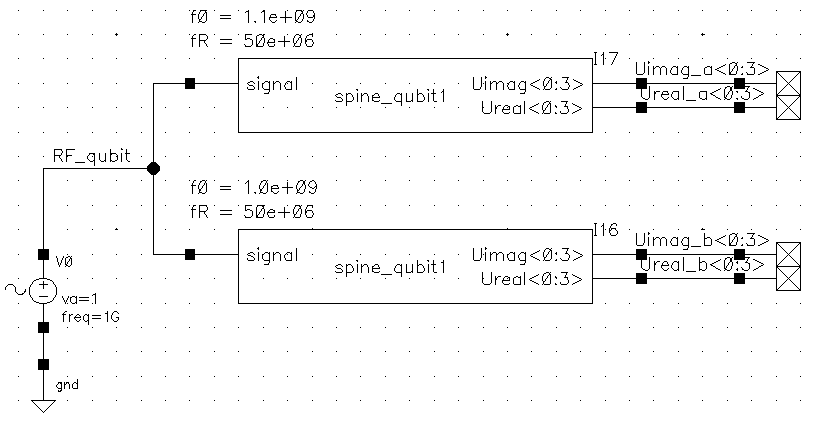
\includegraphics[width=0.6\linewidth]{figures/spine_1_bw.png}
	\caption{Two modules, each emulating one single-electron spin qubit, have been instantiated as a verilog-A module in the electrical circuit simulator; the two qubits are uncoupled and cannot be entangled.}
	\label{fig:spine_spine1}
\end{figure}

\begin{figure}[htbp]
	\centering
	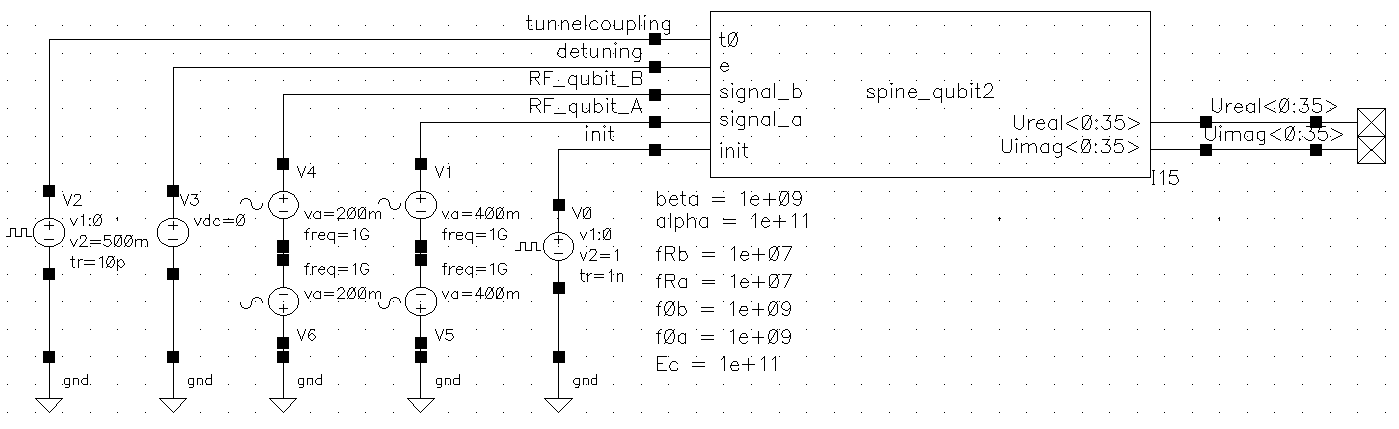
\includegraphics[width=\linewidth]{figures/spine_2_bw.png}
	\caption{A system of two coupled single-electron spin qubits is included as a verilog-A module in the electrical circuit simulator.}
	\label{fig:spine_spine2}
\end{figure}

The inputs to the Verilog-A blocks are the electrical signals applied to the quantum processor (\cref{fig:spine_spine1,fig:spine_spine2}; \texttt{signal} is the RF-signal, \texttt{e} for detuning the quantum dots and \texttt{t0} to control the tunnel coupling) and \texttt{init} to reset the operation to the identity matrix. The resulting complex operation $U$, which can be used to calculate the operation fidelity, is available at the output with separated real (\texttt{Ureal$<>$}) and imaginary (\texttt{Uimag$<>$}) parts in row-major order. Parameters of the physical system are set as a module parameter when instantiating the module in the circuit schematic (\cref{fig:spine_spine1,fig:spine_spine2}; \texttt{Ec} is the charging energy of the quantum dot, \texttt{f0} the spin precession frequency, \texttt{fR} the rotation frequency at 1-V RF-signal, \texttt{beta} the tunnel coupling at \SI{1}{\volt} and \texttt{alpha} the detuning energy at \SI{1}{\volt}).

While the time step control of a transient simulation is managed by the circuit simulator, which relaxes the time step when tolerable, a maximum time step is set by the Verilog-A module to ensure accurate simulation of the quantum physics.

\bibliographystyle{IEEEtran}
\bibliography{spine}

\end{document}